%!TEX root = *.tex
%%%%%%%%%%%%%%%%%%
% メモ
\begin{comment}

\end{comment}
% カウンタのリセット
\setcounter{eqNo}{0}
% 解答
\noindent {\large【解答】\par}

\noindent (1)\par 
\noindent\,(a)\,
反発係数の式より
\begin{align*}
  v_0 = - (v_1-V_1) \assignEqNo
\end{align*}
運動量保存則から
\begin{align*}
  mv_0 = mv_1 + MV_1 \assignEqNo
\end{align*}
\ctext{1},\ctext{2}より
\begin{align*}
  v_1 = \dfrac{m-M}{m+M}v_0,\quad 
  V_1 = \dfrac{2m}{m+M}v_0
\end{align*}

\noindent\,(b)\,
台車に対する小球Aの速度を$u_1$とおくと
\begin{align*}
  u_1 = v_1 - V_1 = -v_0
\end{align*}
であり,台車上でPからQまでの変位$-L$を進むのに要する時間$T$は
$T=\dfrac{L}{v_0}$となる.

さらに,壁Qに衝突するときの反発係数と衝突後の運動量に注目して,
\begin{align*}
  v_1 - V_1 &= - (v_2 -V_2) \assignEqNo\\
  mv_1+MV_1 &= mv_2-MV_2 \assignEqNo
\end{align*}
\ctext{3},\ctext{4}より
\begin{align*}
  v_2 = v_0,\quad V_2 = 0
\end{align*}

{
\begin{wrapfigure}{r}{12zw}
  \vspace{-\intextsep}
  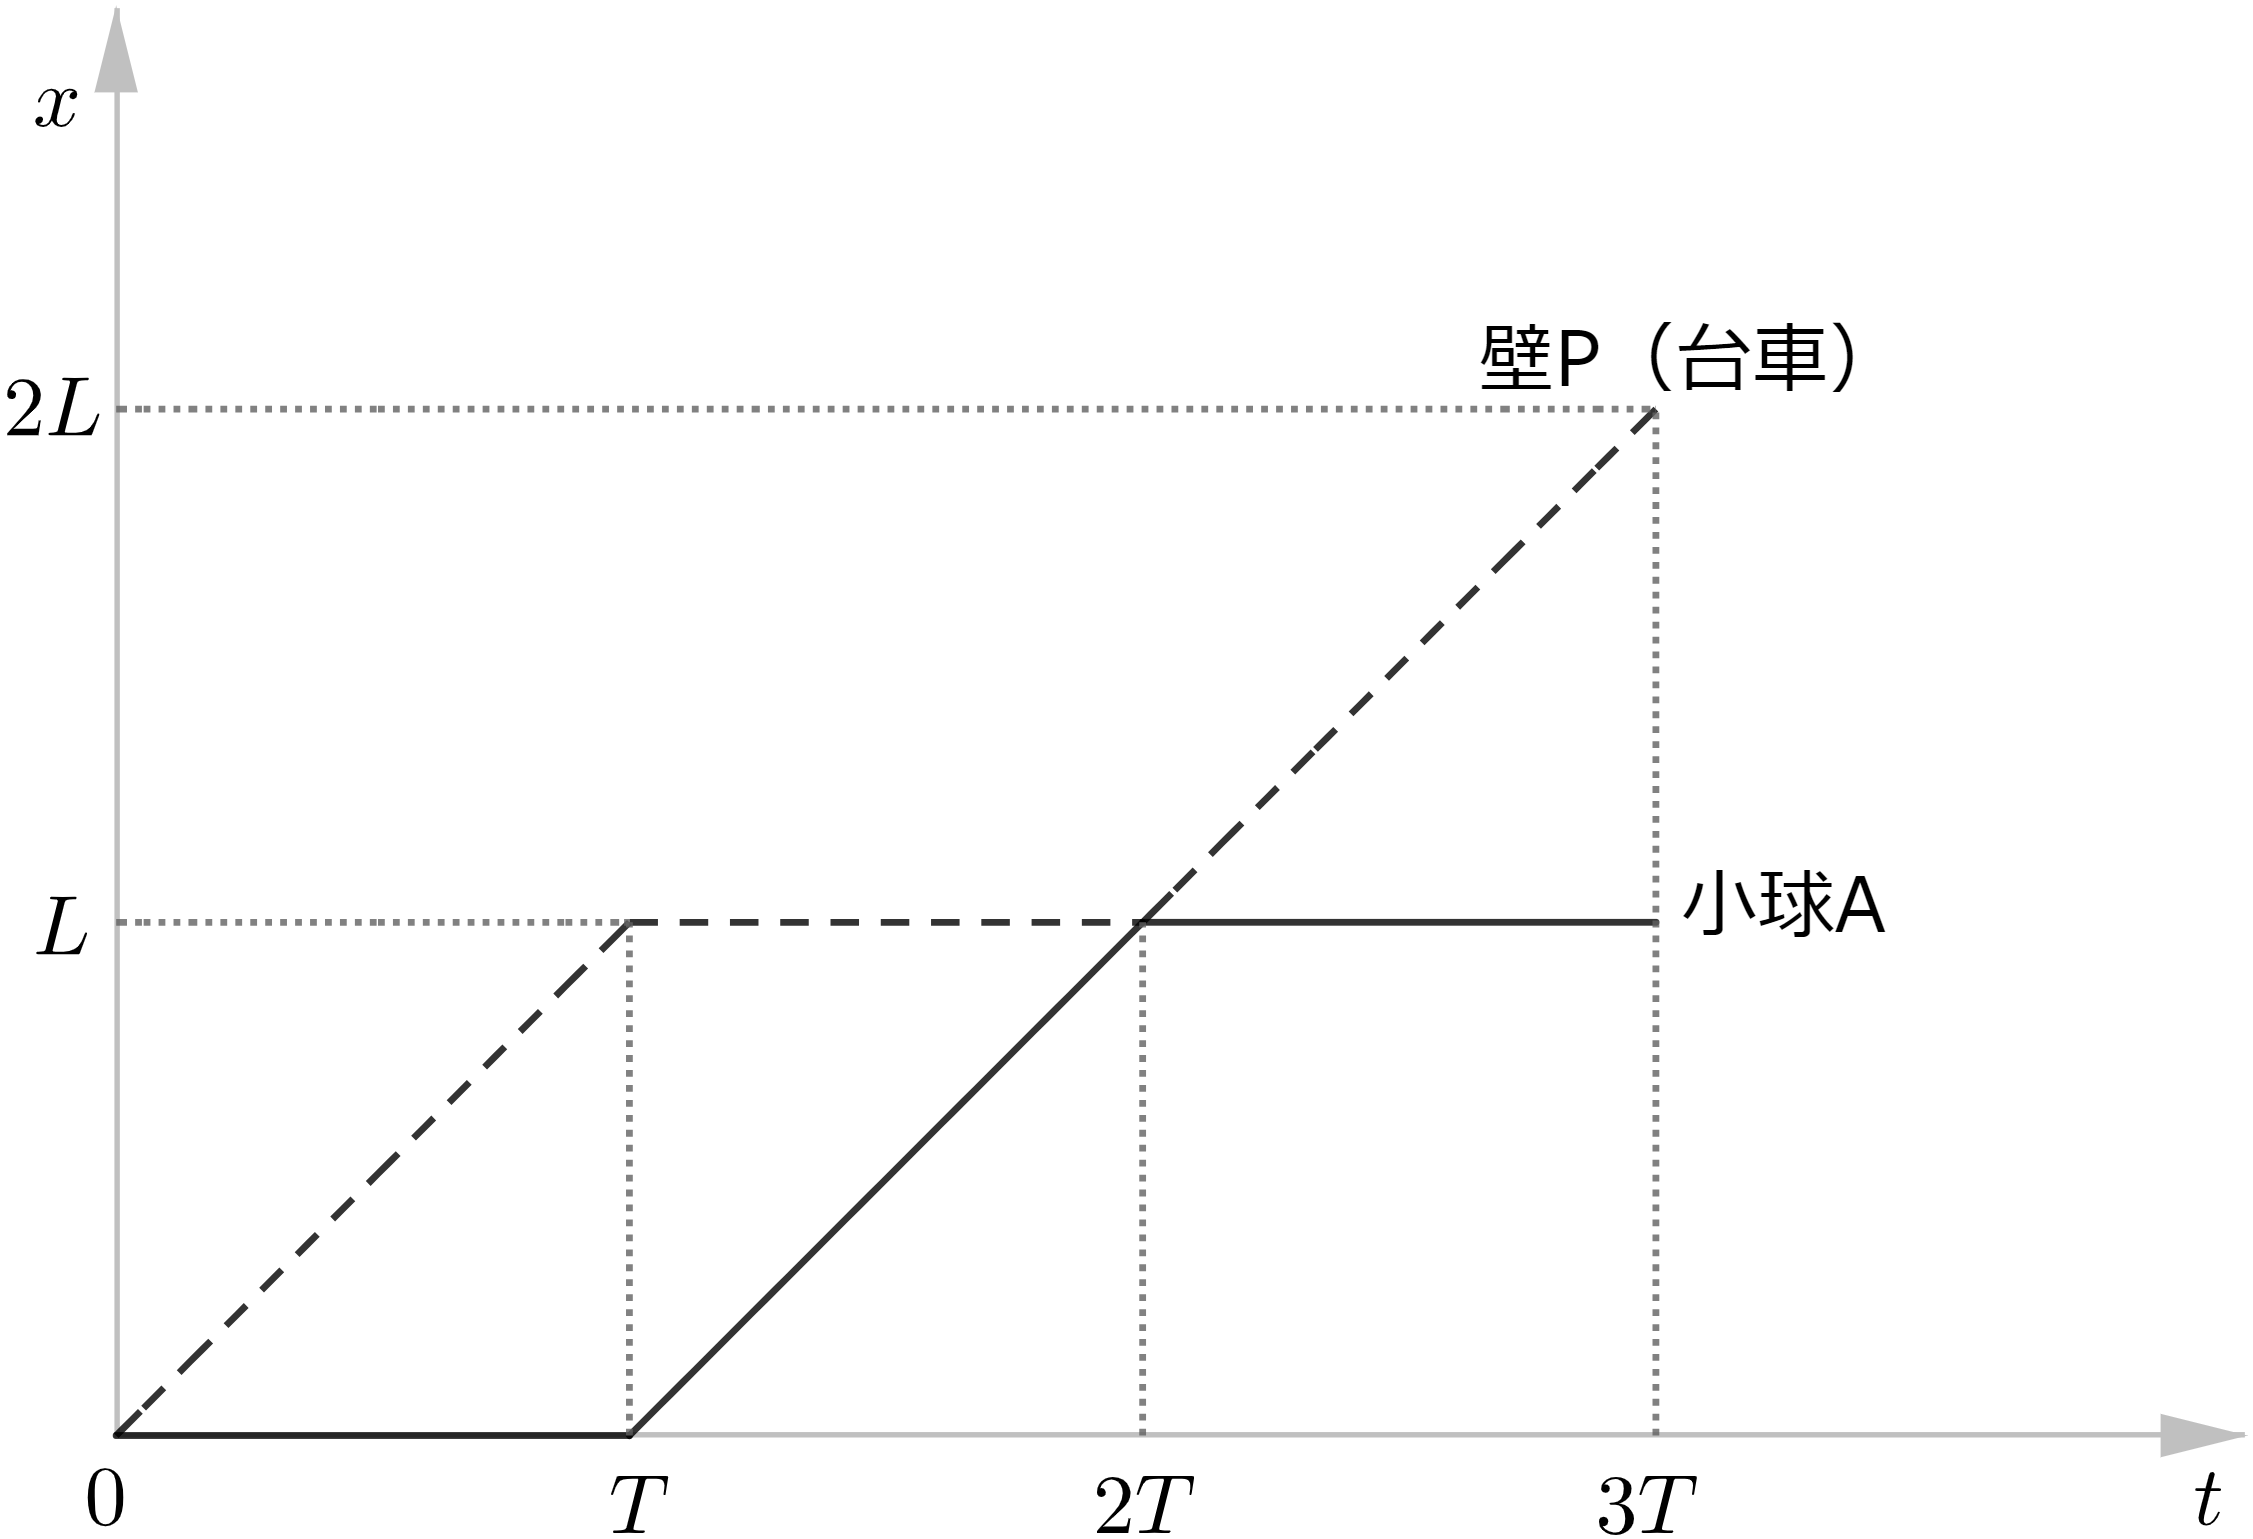
\includegraphics{../graphs/jumon_42_sol.png}
  \caption{}
\end{wrapfigure}

\noindent \,(c)\,
(2)についで,$v_3,\,V_3$を考えると,それぞれ$v_1,\,V_1$に一致する.
したがって,$m$と$M$の関係式によらず台車に対する小球Aの相対速度の大きさは$v_0$で不変であり,衝突の間隔は$T$で一定である.
いま,$m=M$より$v_1=0,\,V_1=v_0$となるので,衝突の度に速度を交換する.
すなわち,小球Aと壁Pの位置の時間変化を$x\mathchar`-t$グラフに表して,図1(右図)を得る.
\par }



\noindent \,(d)\,
$M=2m$とすると
\begin{align*}
  v_1 = -\dfrac{1}{3}v_0,\quad V_1 = \dfrac{2}{3}v_0
\end{align*}
である.
小球AがPで衝突してからQで衝突した後に再びPで衝突するまでの時刻は$2T$であり,
その間に台車が進む距離は
\begin{align*}
  \dfrac{2}{3}v_0 \cdot T = \dfrac{2}{3}L
\end{align*}
である.
また,小球がPQ間を4往復するまでに時間は$8T$かかり,その間に台車は$\dfrac{8}{3}L$進んでいる.
残り$\dfrac{1}{3}L$動くまでの時刻は$\dfrac{(1/3)L}{(2/3)v_0}=\dfrac{1}{2}T$となるので,求める時間は
\begin{align*}
  8T+T=\dfrac{17L}{2v_0}
\end{align*}
である.

\noindent (2)\par 
\noindent\,(a)\,
反発係数の式および運動量保存則より
\begin{align*}
  ev_0 &= -({v_1^\prime}-{V_1}^\prime) \assignEqNo \\
  mv_0 &= m{v_1}^\prime + M{V_1}^\prime \assignEqNo 
\end{align*}
\ctext{5},\ctext{6}より
\begin{align*}
  {v_1}^\prime = \dfrac{m-eM}{m+M}v_0,\quad 
  {V_1}^\prime = \dfrac{(1+e)M}{m+M}v_0
\end{align*}

\noindent\,(b)\,
衝突によって運動量が変わることはないので,
\begin{align*}
  mv_0 = m{v_1}^\prime + M{V_1}^\prime = \cdots = m{v_n}^\prime + M{V_n}^\prime \assignEqNo 
\end{align*}
また,各衝突における反発係数の式は
\begin{align*}
  e=-\dfrac{{v_1}^\prime-{V_1}^\prime}{v_0},\,
  e&=-\dfrac{{v_2}^\prime-{V_2}^\prime}{{v_1}^\prime-{V_1}^\prime},\,
  \cdots ,\, 
  e=-\dfrac{{v_n}^\prime-{V_n}^\prime}{{v_{n-1}}^\prime - {V_{n-1}}^\prime}
  \intertext{これらの辺々をかけ合わせて}
  (-e)^n &= \dfrac{{v_n}^\prime-{V_n}^\prime}{v_0} \assignEqNo
\end{align*}
\ctext{7},\ctext{8}より
\begin{align*}
  {v_n}^\prime = \dfrac{m+(-e)^nM}{m+M}v_0,\quad 
  {V_n}^\prime = \dfrac{\big(1-(-e)^n\big)m}{m+M}v_0
\end{align*}

\noindent\,(c)\, 
$0<e<1$ゆえ$\lim\limits_{n\to\infty}(-e)^n=0$.したがって,
\begin{align*}
  \lim_{n\to\infty}{v_n}^\prime = \dfrac{m}{m+M}v_0,\quad 
  \lim_{n\to\infty}{V_n}^\prime = \dfrac{m}{m+M}v_0
\end{align*}
以上より,十分時間の経過後,
\begin{enumerate}
  \setlength{\leftskip}{0zw}	\setlength{\itemindent}{1zw}
  \setlength{\itemsep}{0.5\baselineskip}
  \setlength{\labelwidth}{0zw}	\setlength{\labelsep}{1zw}
  \item[] 小球は台車と一体となり,速度$\dfrac{m}{m+M}v_0$の等速直線運動を行う.
\end{enumerate}


%%%%%%%%%%%%%%%%%%
